\documentclass[]{book}
\usepackage{lmodern}
\usepackage{amssymb,amsmath}
\usepackage{ifxetex,ifluatex}
\usepackage{fixltx2e} % provides \textsubscript
\ifnum 0\ifxetex 1\fi\ifluatex 1\fi=0 % if pdftex
  \usepackage[T1]{fontenc}
  \usepackage[utf8]{inputenc}
\else % if luatex or xelatex
  \ifxetex
    \usepackage{mathspec}
  \else
    \usepackage{fontspec}
  \fi
  \defaultfontfeatures{Ligatures=TeX,Scale=MatchLowercase}
\fi
% use upquote if available, for straight quotes in verbatim environments
\IfFileExists{upquote.sty}{\usepackage{upquote}}{}
% use microtype if available
\IfFileExists{microtype.sty}{%
\usepackage{microtype}
\UseMicrotypeSet[protrusion]{basicmath} % disable protrusion for tt fonts
}{}
\usepackage[margin=1in]{geometry}
\usepackage{hyperref}
\hypersetup{unicode=true,
            pdftitle={MSDR Package Documentation},
            pdfauthor={AH Uyekita},
            pdfborder={0 0 0},
            breaklinks=true}
\urlstyle{same}  % don't use monospace font for urls
\usepackage{natbib}
\bibliographystyle{apalike}
\usepackage{color}
\usepackage{fancyvrb}
\newcommand{\VerbBar}{|}
\newcommand{\VERB}{\Verb[commandchars=\\\{\}]}
\DefineVerbatimEnvironment{Highlighting}{Verbatim}{commandchars=\\\{\}}
% Add ',fontsize=\small' for more characters per line
\usepackage{framed}
\definecolor{shadecolor}{RGB}{248,248,248}
\newenvironment{Shaded}{\begin{snugshade}}{\end{snugshade}}
\newcommand{\KeywordTok}[1]{\textcolor[rgb]{0.13,0.29,0.53}{\textbf{#1}}}
\newcommand{\DataTypeTok}[1]{\textcolor[rgb]{0.13,0.29,0.53}{#1}}
\newcommand{\DecValTok}[1]{\textcolor[rgb]{0.00,0.00,0.81}{#1}}
\newcommand{\BaseNTok}[1]{\textcolor[rgb]{0.00,0.00,0.81}{#1}}
\newcommand{\FloatTok}[1]{\textcolor[rgb]{0.00,0.00,0.81}{#1}}
\newcommand{\ConstantTok}[1]{\textcolor[rgb]{0.00,0.00,0.00}{#1}}
\newcommand{\CharTok}[1]{\textcolor[rgb]{0.31,0.60,0.02}{#1}}
\newcommand{\SpecialCharTok}[1]{\textcolor[rgb]{0.00,0.00,0.00}{#1}}
\newcommand{\StringTok}[1]{\textcolor[rgb]{0.31,0.60,0.02}{#1}}
\newcommand{\VerbatimStringTok}[1]{\textcolor[rgb]{0.31,0.60,0.02}{#1}}
\newcommand{\SpecialStringTok}[1]{\textcolor[rgb]{0.31,0.60,0.02}{#1}}
\newcommand{\ImportTok}[1]{#1}
\newcommand{\CommentTok}[1]{\textcolor[rgb]{0.56,0.35,0.01}{\textit{#1}}}
\newcommand{\DocumentationTok}[1]{\textcolor[rgb]{0.56,0.35,0.01}{\textbf{\textit{#1}}}}
\newcommand{\AnnotationTok}[1]{\textcolor[rgb]{0.56,0.35,0.01}{\textbf{\textit{#1}}}}
\newcommand{\CommentVarTok}[1]{\textcolor[rgb]{0.56,0.35,0.01}{\textbf{\textit{#1}}}}
\newcommand{\OtherTok}[1]{\textcolor[rgb]{0.56,0.35,0.01}{#1}}
\newcommand{\FunctionTok}[1]{\textcolor[rgb]{0.00,0.00,0.00}{#1}}
\newcommand{\VariableTok}[1]{\textcolor[rgb]{0.00,0.00,0.00}{#1}}
\newcommand{\ControlFlowTok}[1]{\textcolor[rgb]{0.13,0.29,0.53}{\textbf{#1}}}
\newcommand{\OperatorTok}[1]{\textcolor[rgb]{0.81,0.36,0.00}{\textbf{#1}}}
\newcommand{\BuiltInTok}[1]{#1}
\newcommand{\ExtensionTok}[1]{#1}
\newcommand{\PreprocessorTok}[1]{\textcolor[rgb]{0.56,0.35,0.01}{\textit{#1}}}
\newcommand{\AttributeTok}[1]{\textcolor[rgb]{0.77,0.63,0.00}{#1}}
\newcommand{\RegionMarkerTok}[1]{#1}
\newcommand{\InformationTok}[1]{\textcolor[rgb]{0.56,0.35,0.01}{\textbf{\textit{#1}}}}
\newcommand{\WarningTok}[1]{\textcolor[rgb]{0.56,0.35,0.01}{\textbf{\textit{#1}}}}
\newcommand{\AlertTok}[1]{\textcolor[rgb]{0.94,0.16,0.16}{#1}}
\newcommand{\ErrorTok}[1]{\textcolor[rgb]{0.64,0.00,0.00}{\textbf{#1}}}
\newcommand{\NormalTok}[1]{#1}
\usepackage{longtable,booktabs}
\usepackage{graphicx,grffile}
\makeatletter
\def\maxwidth{\ifdim\Gin@nat@width>\linewidth\linewidth\else\Gin@nat@width\fi}
\def\maxheight{\ifdim\Gin@nat@height>\textheight\textheight\else\Gin@nat@height\fi}
\makeatother
% Scale images if necessary, so that they will not overflow the page
% margins by default, and it is still possible to overwrite the defaults
% using explicit options in \includegraphics[width, height, ...]{}
\setkeys{Gin}{width=\maxwidth,height=\maxheight,keepaspectratio}
\IfFileExists{parskip.sty}{%
\usepackage{parskip}
}{% else
\setlength{\parindent}{0pt}
\setlength{\parskip}{6pt plus 2pt minus 1pt}
}
\setlength{\emergencystretch}{3em}  % prevent overfull lines
\providecommand{\tightlist}{%
  \setlength{\itemsep}{0pt}\setlength{\parskip}{0pt}}
\setcounter{secnumdepth}{5}
% Redefines (sub)paragraphs to behave more like sections
\ifx\paragraph\undefined\else
\let\oldparagraph\paragraph
\renewcommand{\paragraph}[1]{\oldparagraph{#1}\mbox{}}
\fi
\ifx\subparagraph\undefined\else
\let\oldsubparagraph\subparagraph
\renewcommand{\subparagraph}[1]{\oldsubparagraph{#1}\mbox{}}
\fi

%%% Use protect on footnotes to avoid problems with footnotes in titles
\let\rmarkdownfootnote\footnote%
\def\footnote{\protect\rmarkdownfootnote}

%%% Change title format to be more compact
\usepackage{titling}

% Create subtitle command for use in maketitle
\newcommand{\subtitle}[1]{
  \posttitle{
    \begin{center}\large#1\end{center}
    }
}

\setlength{\droptitle}{-2em}

  \title{MSDR Package Documentation}
    \pretitle{\vspace{\droptitle}\centering\huge}
  \posttitle{\par}
    \author{AH Uyekita}
    \preauthor{\centering\large\emph}
  \postauthor{\par}
      \predate{\centering\large\emph}
  \postdate{\par}
    \date{2019-02-21}

\usepackage{booktabs}

\begin{document}
\maketitle

{
\setcounter{tocdepth}{1}
\tableofcontents
}
\chapter*{Prerequisites}\label{prerequisites}
\addcontentsline{toc}{chapter}{Prerequisites}

This is a \emph{sample} book written in \textbf{Markdown}. You can use
anything that Pandoc's Markdown supports, e.g., a math equation
\(a^2 + b^2 = c^2\).

The \textbf{bookdown} package can be installed from CRAN or Github:

\begin{Shaded}
\begin{Highlighting}[]
\KeywordTok{install.packages}\NormalTok{(}\StringTok{"bookdown"}\NormalTok{)}
\CommentTok{# or the development version}
\CommentTok{# devtools::install_github("rstudio/bookdown")}
\end{Highlighting}
\end{Shaded}

Remember each Rmd file contains one and only one chapter, and a chapter
is defined by the first-level heading \texttt{\#}.

To compile this example to PDF, you need XeLaTeX. You are recommended to
install TinyTeX (which includes XeLaTeX):
\url{https://yihui.name/tinytex/}.

\chapter{eq\_clean\_data}\label{eq_clean_data}

This function has two behaviours:

\begin{enumerate}
\def\labelenumi{\arabic{enumi})}
\tightlist
\item
  When you assign a file to load, and;
\end{enumerate}

\begin{Shaded}
\begin{Highlighting}[]
\CommentTok{# Loading the 'signif.txt' file.}
\KeywordTok{eq_clean_data}\NormalTok{(}\DataTypeTok{file_name =} \KeywordTok{system.file}\NormalTok{(}\StringTok{"extdata"}\NormalTok{, }\StringTok{"signif.txt"}\NormalTok{, }\DataTypeTok{package =} \StringTok{"msdr"}\NormalTok{))}
\end{Highlighting}
\end{Shaded}

\begin{enumerate}
\def\labelenumi{\arabic{enumi})}
\setcounter{enumi}{1}
\tightlist
\item
  When you pipe a dataset already loaded.
\end{enumerate}

\begin{Shaded}
\begin{Highlighting}[]
\CommentTok{# Pipe.}
\NormalTok{readr}\OperatorTok{::}\KeywordTok{read_delim}\NormalTok{(}\StringTok{"signif.txt"}\NormalTok{,}
                  \DataTypeTok{delim =} \StringTok{"}\CharTok{\textbackslash{}t}\StringTok{"}\NormalTok{) }\OperatorTok\StringTok{ }\KeywordTok{eq_clean_data}\NormalTok{()}
\end{Highlighting}
\end{Shaded}

\section{Loading the data}\label{load_data}

This function also loads the Earthquake database from NOAA.

I\_D

YEAR

LOCATION\_NAME

EQ\_PRIMARY

TOTAL\_DEATHS

1

-2150

JORDAN: BAB-A-DARAA,AL-KARAK

7.3

NA

3

-2000

TURKMENISTAN: W

7.1

1

2

-2000

SYRIA: UGARIT

NA

NA

5877

-1610

GREECE: THERA ISLAND (SANTORINI)

NA

NA

8

-1566

ISRAEL: ARIHA (JERICHO)

NA

NA

11

-1450

ITALY: LACUS CIMINI

NA

NA

As you can see, there are several observations with NA values.

\section{Creating new features}\label{new_features}

The \texttt{eq\_clean\_data} creates the DATE variable binding the
columns YEAR, MONTH, and DAY. All this using the
\href{https://lubridate.tidyverse.org}{Lubridate} package.

\begin{Shaded}
\begin{Highlighting}[]
\CommentTok{# Creating a new feature.}
\NormalTok{df <-}\StringTok{ }\NormalTok{df }\OperatorTok
\StringTok{       }\KeywordTok{mutate}\NormalTok{(}\DataTypeTok{DATE =}\NormalTok{ lubridate}\OperatorTok{::}\KeywordTok{ymd}\NormalTok{(}\KeywordTok{paste}\NormalTok{(df}\OperatorTok{$}\NormalTok{YEAR,      }\CommentTok{# YEAR column}
\NormalTok{                                          df}\OperatorTok{$}\NormalTok{MONTH,     }\CommentTok{# MONTH column}
\NormalTok{                                          df}\OperatorTok{$}\NormalTok{DAY,       }\CommentTok{# DAY column}
                                          \DataTypeTok{sep =} \StringTok{"/"}\NormalTok{)))  }\CommentTok{# YYYY/MM/DD}
\end{Highlighting}
\end{Shaded}

\section{Conversion Process}\label{conversion}

I have converted the class of some features:

\begin{itemize}
\tightlist
\item
  \texttt{TOTAL\_DEATHS} to numeric;
\item
  \texttt{EQ\_PRIMARY} to numeric;
\item
  All \texttt{NA}'s of \texttt{TOTAL\_DEATHS} in zeros.
\end{itemize}

\section{Cleaning Process}\label{cleaning}

I have removed:

\begin{itemize}
\tightlist
\item
  All observations flagged as Tsunami, and;
\item
  All observations with no Date.
\end{itemize}

\section{Example 1}\label{example_1}

How to load a \texttt{txt} file.

\begin{Shaded}
\begin{Highlighting}[]

\CommentTok{# Load the package}
\KeywordTok{library}\NormalTok{(msdr)}

\CommentTok{# Define as file_name the txt file.}
\NormalTok{df <-}\StringTok{ }\KeywordTok{eq_clean_data}\NormalTok{(}\DataTypeTok{file_name =}\NormalTok{ raw_data_path)}

\CommentTok{# Dimensions of the loaded dataframe.}
\KeywordTok{dim}\NormalTok{(df)}
\CommentTok{#> [1] 2840   49}
\end{Highlighting}
\end{Shaded}

\section{Example 2}\label{example_2}

Piping a dataset to the \texttt{eq\_clean\_data}.

\begin{Shaded}
\begin{Highlighting}[]

\CommentTok{# Load the package}
\KeywordTok{library}\NormalTok{(msdr)}

\CommentTok{# Piping a read_delim with eq_clean_data.}
\NormalTok{readr}\OperatorTok{::}\KeywordTok{read_delim}\NormalTok{(raw_data_path,}
                  \DataTypeTok{delim =} \StringTok{"}\CharTok{\textbackslash{}t}\StringTok{"}\NormalTok{) }\OperatorTok
\StringTok{       }
\StringTok{              }\KeywordTok{eq_clean_data}\NormalTok{() ->}\StringTok{ }\NormalTok{df}

\CommentTok{# Dimensions of the loaded dataframe.}
\KeywordTok{dim}\NormalTok{(df)}
\CommentTok{#> [1] 2840   49}
\end{Highlighting}
\end{Shaded}

\chapter{eq\_location\_clean}\label{eq_location_clean}

\section{Introduction}\label{intro}

This function creates a new column with the earthquake
\texttt{LOCATION}. The function \texttt{eq\_clean\_data} uses it behind
the scenes, so it is not necessary to call this function after call
\texttt{eq\_clean\_data}.

\section{Example}\label{example}

Piping a raw data to creates a LOCATION column.

\begin{Shaded}
\begin{Highlighting}[]
\CommentTok{# Path to the raw data.}
\NormalTok{raw_data_path <-}\StringTok{ }\KeywordTok{system.file}\NormalTok{(}\StringTok{"extdata"}\NormalTok{, }\StringTok{"signif.txt"}\NormalTok{, }\DataTypeTok{package =} \StringTok{"msdr"}\NormalTok{)}

\CommentTok{# Loading the dataset of Earthquake.}
\NormalTok{df <-}\StringTok{ }\NormalTok{readr}\OperatorTok{::}\KeywordTok{read_delim}\NormalTok{(}\DataTypeTok{file =}\NormalTok{ raw_data_path,      }
                        \DataTypeTok{delim =} \StringTok{'}\CharTok{\textbackslash{}t}\StringTok{'}\NormalTok{,              }
                        \DataTypeTok{col_names =} \OtherTok{TRUE}\NormalTok{,          }
                        \DataTypeTok{progress =} \OtherTok{FALSE}\NormalTok{,           }
                        \DataTypeTok{col_types =}\NormalTok{ readr}\OperatorTok{::}\KeywordTok{cols}\NormalTok{())}

\CommentTok{# Printing some columns.}
\NormalTok{df }\OperatorTok
\StringTok{       }\KeywordTok{eq_location_clean}\NormalTok{() }\OperatorTok
\StringTok{              }\CommentTok{# Selecting some features.}
\StringTok{              }\KeywordTok{select}\NormalTok{(YEAR,}
\NormalTok{                     COUNTRY,}
\NormalTok{                     LOCATION,}
\NormalTok{                     EQ_PRIMARY,}
\NormalTok{                     TOTAL_DEATHS) }\OperatorTok\StringTok{ }
\StringTok{                     }\CommentTok{# Filtering.}
\StringTok{                     }\KeywordTok{filter}\NormalTok{(YEAR }\OperatorTok{>}\StringTok{ }\DecValTok{1990} \OperatorTok{&}
\StringTok{                            }\NormalTok{YEAR }\OperatorTok{<}\StringTok{ }\DecValTok{2019}\NormalTok{) }\OperatorTok
\StringTok{                            }\CommentTok{# Show the first 10 rows.}
\StringTok{                            }\KeywordTok{head}\NormalTok{(}\DecValTok{10}\NormalTok{) }\OperatorTok
\StringTok{                                   }\CommentTok{# Enhance table visualization.}
\StringTok{                                   }\KeywordTok{kable}\NormalTok{()}
\end{Highlighting}
\end{Shaded}

YEAR

COUNTRY

LOCATION

EQ\_PRIMARY

TOTAL\_DEATHS

1991

MYANMAR (BURMA)

Thabeikkyin, Mandalay

7.1

NA

1991

AFGHANISTAN

Badakhstan, Baghlan, Laghman, Nagarhar

6.4

848

1991

SOLOMON ISLANDS

Solomon Islands

6.9

NA

1991

FRANCE

France

3.8

9

1991

RUSSIA

Kuril Islands

5.7

NA

1991

BERING SEA

Bering Sea

6.7

NA

1991

CHINA

Kalpin

6.1

NA

1991

CHINA

Ne, Datong

5.5

NA

1991

PERU

Rioja, Neuva Cajamarca

6.4

NA

1991

PERU

Rioja, Moyobamba, Nueva Cajamarca

6.7

53

As you can see, the \texttt{LOCATION} column has only cities in Title
Case mode.

\chapter{geom\_timeline}\label{geom_timeline}

The \texttt{geom\_timeline} is a new \texttt{geom\_*} of
\texttt{ggplot2} package that aims to enhance the visualization of
earthquake. This Geom has some configuration:

\begin{itemize}
\tightlist
\item
  size: The earthquakes as displayed as circles with different radius
  (according to the \texttt{EQ\_PRIMARY});
\item
  color: This is based on the \texttt{TOTAL\_DEATHS};
\item
  x axis: This is the temporal axis.
\item
  y axis: Each county has your own line, it is not possible to mix
  countries in a single y axis.
\end{itemize}

\section{Example 1}\label{example_1}

Let's plot the earthquake from 1000 to 2000, which occured in
\texttt{JAPAN}.

\begin{Shaded}
\begin{Highlighting}[]
\CommentTok{# Path to the raw data.}
\NormalTok{raw_data_path <-}\StringTok{ }\KeywordTok{system.file}\NormalTok{(}\StringTok{"extdata"}\NormalTok{, }\StringTok{"signif.txt"}\NormalTok{, }\DataTypeTok{package =} \StringTok{"msdr"}\NormalTok{)}

\CommentTok{# Loading the dataset of Earthquake.}
\NormalTok{df <-}\StringTok{ }\NormalTok{readr}\OperatorTok{::}\KeywordTok{read_delim}\NormalTok{(}\DataTypeTok{file =}\NormalTok{ raw_data_path,      }
                        \DataTypeTok{delim =} \StringTok{'}\CharTok{\textbackslash{}t}\StringTok{'}\NormalTok{,              }
                        \DataTypeTok{col_names =} \OtherTok{TRUE}\NormalTok{,          }
                        \DataTypeTok{progress =} \OtherTok{FALSE}\NormalTok{,           }
                        \DataTypeTok{col_types =}\NormalTok{ readr}\OperatorTok{::}\KeywordTok{cols}\NormalTok{())}

\CommentTok{# Cleaning the data and filtering.}
\NormalTok{df }\OperatorTok\StringTok{ }
\StringTok{       }\KeywordTok{eq_clean_data}\NormalTok{() }\OperatorTok
\StringTok{       }
\StringTok{              }\KeywordTok{filter}\NormalTok{(COUNTRY }\OperatorTok\StringTok{ 'JAPAN'}\NormalTok{,}
\NormalTok{                     YEAR }\OperatorTok{>=}\StringTok{ }\DecValTok{1000} \OperatorTok{&}
\StringTok{                     }\NormalTok{YEAR }\OperatorTok{<=}\StringTok{ }\DecValTok{2000}\NormalTok{) }\OperatorTok
\StringTok{              }\CommentTok{# Creating a ggplot object}
\StringTok{              }\KeywordTok{ggplot}\NormalTok{() }\OperatorTok{+}\StringTok{ }
\StringTok{                     }\CommentTok{# Using the new Geom}
\StringTok{                     }\KeywordTok{geom_timeline}\NormalTok{(}\KeywordTok{aes}\NormalTok{(}\DataTypeTok{x     =}\NormalTok{ DATE,}
                                       \DataTypeTok{y     =}\NormalTok{ COUNTRY,}
                                       \DataTypeTok{size  =}\NormalTok{ EQ_PRIMARY,}
                                       \DataTypeTok{color =}\NormalTok{ TOTAL_DEATHS)) }\OperatorTok{+}
\StringTok{                            }\CommentTok{# Adding theme.}
\StringTok{                            }\KeywordTok{theme_msdr}\NormalTok{() }\OperatorTok{+}\StringTok{ }
\StringTok{                                   }\CommentTok{# Editing the legends' titles }
\StringTok{                                   }\KeywordTok{labs}\NormalTok{(}\DataTypeTok{size =} \StringTok{"Richter scale value"}\NormalTok{,}
                                        \DataTypeTok{color =} \StringTok{"# deaths"}\NormalTok{)}
\end{Highlighting}
\end{Shaded}

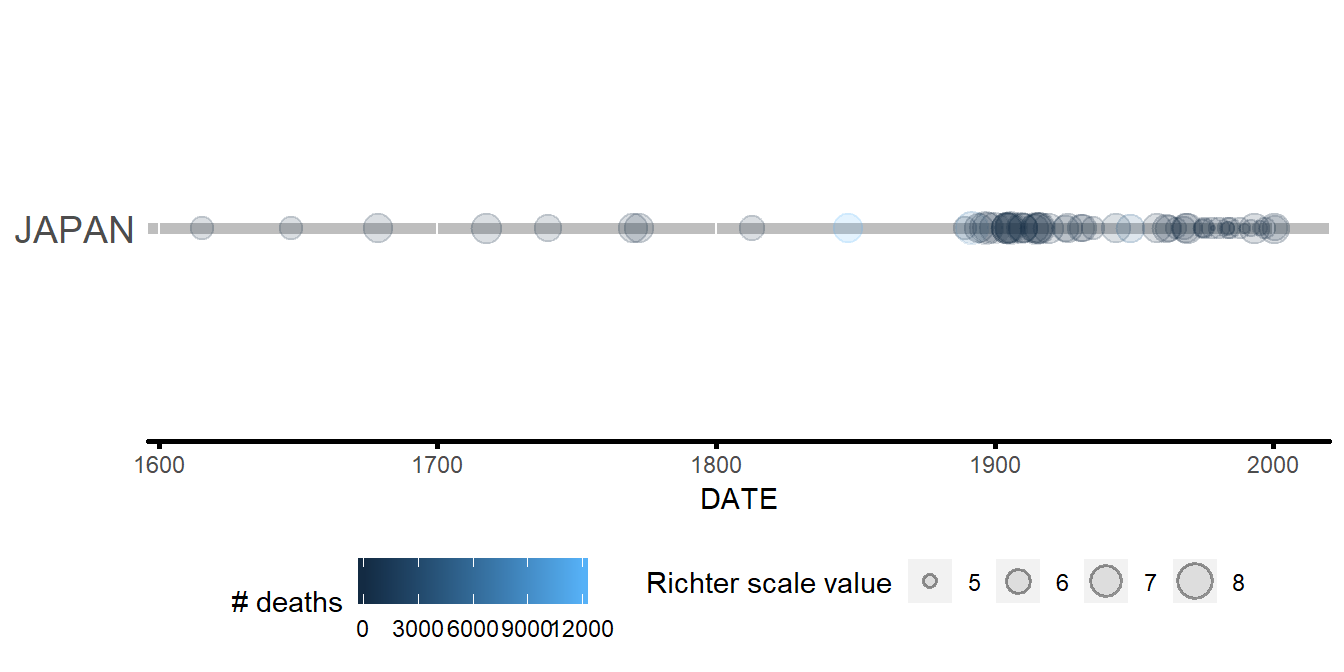
\includegraphics[width=1\linewidth]{MSDR_Capstone_files/figure-latex/unnamed-chunk-17-1}

Most of earthquake records in Japan are concentrated between 1900 and
2000.

\section{Example 2}\label{example_2}

The earthquake record of 2018. Simple comparison.

\begin{Shaded}
\begin{Highlighting}[]
\CommentTok{# List of countries in Europe and "West Asia". This is not an exhaustive list.}
\NormalTok{eurasia <-}\StringTok{ }\KeywordTok{c}\NormalTok{(}\StringTok{'SPAIN'}\NormalTok{,}\StringTok{'GREECE'}\NormalTok{,}\StringTok{'TURKEY'}\NormalTok{,}\StringTok{'PORTUGAL'}\NormalTok{,}\StringTok{'RUSSIA'}\NormalTok{,}\StringTok{'FRANCE'}\NormalTok{,}\StringTok{'MACEDONIA'}\NormalTok{,}\StringTok{'BULGARIA'}\NormalTok{,}
             \StringTok{'ALBANIA'}\NormalTok{,}\StringTok{'GEORGIA'}\NormalTok{,}\StringTok{'ITALY'}\NormalTok{,}\StringTok{'SLOVENIA'}\NormalTok{,}\StringTok{'UK'}\NormalTok{,}\StringTok{'CYPRUS'}\NormalTok{,}\StringTok{'UKRAINE'}\NormalTok{,}\StringTok{'CROATIA'}\NormalTok{,}\StringTok{'AUSTRIA'}\NormalTok{)}

\CommentTok{# Cleaninig data and filtering.}
\NormalTok{df }\OperatorTok\StringTok{ }
\StringTok{       }\KeywordTok{eq_clean_data}\NormalTok{() }\OperatorTok
\StringTok{              }\CommentTok{# Creating a new feature.}
\StringTok{              }\KeywordTok{mutate}\NormalTok{(}\DataTypeTok{CONTINENT =} \KeywordTok{case_when}\NormalTok{(COUNTRY }\OperatorTok\StringTok{ }\NormalTok{eurasia }\OperatorTok{~}\StringTok{ "EURASIA"}\NormalTok{,}
                                          \OperatorTok{!}\NormalTok{(COUNTRY }\OperatorTok\StringTok{ }\NormalTok{eurasia) }\OperatorTok{~}\StringTok{ "WORLD"}\NormalTok{)) }\OperatorTok
\StringTok{                     }\CommentTok{# Filtering.}
\StringTok{                     }\KeywordTok{filter}\NormalTok{(YEAR }\OperatorTok{>=}\StringTok{ }\DecValTok{2018} \OperatorTok{&}
\StringTok{                            }\NormalTok{YEAR }\OperatorTok{<=}\StringTok{ }\DecValTok{2019}\NormalTok{) }\OperatorTok
\StringTok{              }
\StringTok{                            }\CommentTok{# Creating a ggplot object}
\StringTok{                            }\KeywordTok{ggplot}\NormalTok{() }\OperatorTok{+}\StringTok{ }
\StringTok{                                   }\CommentTok{# Using the new Geom}
\StringTok{                                   }\KeywordTok{geom_timeline}\NormalTok{(}\KeywordTok{aes}\NormalTok{(}\DataTypeTok{x     =}\NormalTok{ DATE,}
                                                     \DataTypeTok{y     =}\NormalTok{ CONTINENT,}
                                                     \DataTypeTok{size  =}\NormalTok{ EQ_PRIMARY,}
                                                     \DataTypeTok{color =}\NormalTok{ TOTAL_DEATHS)) }\OperatorTok{+}
\StringTok{                                          }\CommentTok{# Adding theme.}
\StringTok{                                          }\KeywordTok{theme_msdr}\NormalTok{() }\OperatorTok{+}\StringTok{ }
\StringTok{                                                 }\CommentTok{# Editing the legends' titles }
\StringTok{                                                 }\KeywordTok{labs}\NormalTok{(}\DataTypeTok{size =} \StringTok{"Richter scale value"}\NormalTok{,}
                                                      \DataTypeTok{color =} \StringTok{"# deaths"}\NormalTok{)}
\end{Highlighting}
\end{Shaded}

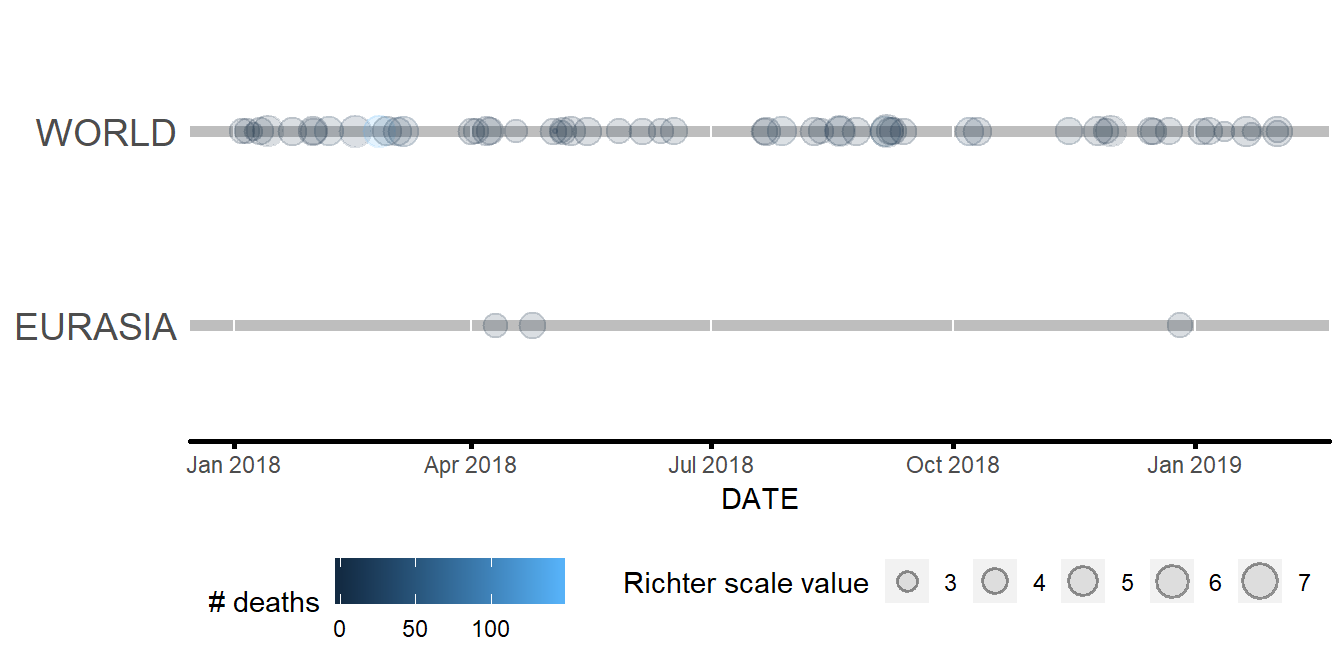
\includegraphics{MSDR_Capstone_files/figure-latex/unnamed-chunk-18-1.pdf}

\bibliography{book.bib,packages.bib}


\end{document}
